%%%% 補助スライド
\appendix
\backupbegin

\begin{frame}{~}
 \centering
 - 補足用 -
\end{frame} 

%%%%%%%%%%%%%%%%%%%%%%%%%%%%%%%%%%%%%%%%%%%%%%%%%%
%% 改良符号化 (根付き連結制約)
%%%%%%%%%%%%%%%%%%%%%%%%%%%%%%%%%%%%%%%%%%%%%%%%%%
\begin{frame}[fragile]{根付き連結制約}
\begin{exampleblock}{基本符号化}\small
\begin{lstlisting}
(1) :- node(X),  not reached(X,_).
(2) :- reached(X,R1), reached(X,R2), R1 < R2.
\end{lstlisting}
\end{exampleblock}
\vfill
\begin{itemize}
\item (1) 各ノード\code{X}について,\structure{\bf 少なくとも1つ}の根から到達可能であることを意味する.
      \structure{\bf (at-least-one制約)}
\item (2) 各ノード\code{X}について,\structure{\bf 高々1つ}の根から到達可能であることを意味する.
      \structure{\bf (at-most-one制約)}
\end{itemize}
\begin{exampleblock}{改良符号化}\small
\begin{lstlisting}
(3) :- node(X), not 1 { reached(X,R) } 1.
\end{lstlisting}
\end{exampleblock}
\vfill
\begin{itemize}
\item (3) 各ノード\code{X}について,ちょうど1つの根からのみ到達可能であることを意味する.
\end{itemize}
\end{frame}

%%%%%%%%%%%%%%%%%%%%%%%%%%%%%%%%%%%%%%%%%%%%%%%%%%
%% 電気制約
%%%%%%%%%%%%%%%%%%%%%%%%%%%%%%%%%%%%%%%%%%%%%%%%%%
\begin{frame}{電気制約の効率的な実装}
 \begin{itemize}
  \item \alert{\bf 電気制約}は,送電する電流$\cdot$電圧の適正範囲を保証する制約.
  \begin{itemize}
   \item 供給経路の各区間で許容電流を超えない.
   \item 電気抵抗による電圧降下が許容範囲を超えない.
   \item etc.
  \end{itemize}
  \item 電流と電圧が影響し合う\structure{\bf 実数ドメイン上の制約}によって表される.
  \item 実数ドメイン上の制約は,純粋なASPのみで扱うのは\alert{\bf 困難}.
		\begin{itemize}
		 \item \structure{\bf 方針1:} 簡易的な電流の電気制約について実装する.
		 \item \structure{\bf 方針2:} ASPMT技術により,背景理論ソルバーと連携して厳密に\\
               \hspace{4zw}\!電流・電圧の制約を実装する.
		\end{itemize}
 \end{itemize}
\end{frame}
%%%%%%%%%%%%%%%%%%%%%%%%%%%%%%%%%%%%%%%%%%%%%%%%%%
%% 電気制約 方針
%%%%%%%%%%%%%%%%%%%%%%%%%%%%%%%%%%%%%%%%%%%%%%%%%%
\begin{frame}{電気制約 方針1}
 \begin{itemize}
  \item 変電所を定電流源と仮定すると,各配電区間での電流の大きさは\structure{\bf 一定の値}として表される.
  \item 供給経路が決まると,ある配電区間に流れる電流は,その配電区間以下の
		電流の大きさの\alert{\bf 線形和}として表すことができる.
  \item グラフでの直感的な意味は,各連結成分の\structure{\bf 根からの深さ}が大きくなるほど,
		上流での電流は大きくなることを意味する.
  \item 根からの深さを表す変数を導入することで,
		各区間に流れる電流の値を計算することができ,\structure{\bf 電流の電気制約には対応可能}.
		\begin{itemize}
		 \item 実際には配電システム(三相交流)についての特殊な計算が必要.
		\end{itemize}
 \end{itemize}\vfill
 \begin{exampleblock}{電流の計算例}
  \centering
  %%%%%%%%%%%%%%%%%%%%%%%%%%%%%%%%%%%%%%%%%%%%%%%%%%
% 電気制約の例
%%%%%%%%%%%%%%%%%%%%%%%%%%%%%%%%%%%%%%%%%%%%%%%%%%

\begin{tikzpicture}[scale=0.5]

 % 設定
 \tikzset{node/.style={rectangle, draw=black,fill=white}}

 \definecolor{edge1}{RGB}{191,0,0}
 \definecolor{node1}{RGB}{249,200,200}
 \definecolor{edge3}{RGB}{38,38,134}
 \definecolor{node3}{RGB}{200,200,249}

 % 補助線
 % \draw [help lines,blue] (0,0) grid (20,6);

 % node %
 \node[circle, ultra thick, draw=edge1, fill=node1,minimum size=1cm](1){};
 \node[node, thick, fill=node1, draw=edge1, right=2.5cm of 1] (2){};
 \node[node, thick, fill=node1, draw=edge1, right=3cm of 2] (3){};
 \node[node, thick, fill=node1, draw=edge1, right=2.5cm of 3] (4){};

 % 変電所 %
 \begin{scope}[scale=1.5]
 \draw [ultra thick, draw=edge1] (0,0) circle [radius=0.225cm] node[minimum size=0.5cm](root1){};
 \draw [ultra thick, draw=edge1] (0.225,0)--(0.35,0)--(0.35,0.35);
 \draw [ultra thick, draw=edge1] (-0.225,0)--(-0.35,0)--(-0.35,-0.35);
 \draw [ultra thick, draw=edge1] (0,0.225)--(0,0.35);
 \draw [ultra thick, draw=edge1] (0,-0.225)--(0,-0.35);
 \draw [ultra thick, draw=edge1] [domain=-0.284:-0.159] plot(\x,\x);
 \draw [ultra thick, draw=edge1] [domain=0.159:0.284] plot(\x,\x);
 \draw [ultra thick, draw=edge1] [domain=-0.284:-0.159] plot(\x,-\x);
 \draw [ultra thick, draw=edge1] [domain=0.159:0.284] plot(\x,-\x);
 \end{scope}

 \draw [line width=3.5pt, edge1] (1) -- %
 node[above, font=\Large, label=below:\color{black}{$I_i\colon\quad$30A}]
 {\textbf{$J_i\colon\quad$\!\!60A}}(5,0) -- (2);
 
 \draw [line width=2.5pt, edge1] (2) -- %
 node[above, font=\Large, label=below:\color{black}{20A}] {\textbf{30A}}(11,0) -- (3);

 \draw [line width=1.5pt, edge1] (3) -- %
 node[above, font=\large, label=below:\color{black}{10A}] {\textbf{10A}}(17,0) -- (4);

\end{tikzpicture}

%%%%%%%%%%%%%%%%%%%%%%%%%%%%%%%%%%%%%%%%%%%%%%%%%%%%%%%%%%
%%% Local Variables:
%%% mode: japanese-latex
%%% TeX-master: ``slide''
%%% End:

 \end{exampleblock} \vfill
\end{frame}
%%%%%%%%%%%%%%%%%%%%%%%%%%%%%%%%%%%%%%%%%%%%%%%%%%
%% 解の遷移問題
%%%%%%%%%%%%%%%%%%%%%%%%%%%%%%%%%%%%%%%%%%%%%%%%%%
\begin{frame}{配電網問題の解の遷移問題への拡張(1/2)}
 \begin{itemize}
  \item 配電網の構成制御における障害時のスイッチの切替手順を求める問題に応用できる.
  \item トポロジ制約のみの場合,ある配電網構成(スタート状態)から,他の配電網構成(ゴール状態)への
        スイッチの切替手順を求める解の遷移問題は,\alert{\bf 根付き全域森遷移問題}に帰着できる.
 \end{itemize}
 \begin{block}{根付き全域森遷移問題}
  根付き全域森問題とその2つの実行可能解が与えられたとき,
  ある解から他のもう一つの解へ,遷移制約を満たしながら,実行可能解のみを経由して到達できるか
  どうかを判定する\alert{\bf 解の遷移問題}.
  \begin{itemize}
  \item 各ステップ$t$で変更可能な辺の数を$d$個以下に制限.(\textbf{遷移制約})
  \item 最短ステップ長での辺の変更手順を求めることが目的となる.
  \end{itemize}
 \end{block} 
\end{frame}
%%%%%%%%%%%%%%%%%%%%%%%%%%%%%%%%%%%%%%%%%%%%%%%%%%
%% 提案アプローチ
%%%%%%%%%%%%%%%%%%%%%%%%%%%%%%%%%%%%%%%%%%%%%%%%%%
\begin{frame}{配電網問題の解の遷移問題への拡張(2/2)}
 \begin{itemize}
  \item 根付き全域森遷移問題のASP符号化を2種類考案した.
 \end{itemize}
 \begin{block}{シングルショット符号化 (改良符号化の自然な拡張)}
    \begin{itemize}
    \item 与えられたステップ長$t$の解が存在するかを判定する.
      % \begin{itemize}
      % \item 与えられたステップ長$t$の解が存在するかを判定する.
      % \item 各アトムにステップ長を表す項\code{T}を追加.例) \code{inForest(X,Y,T)}
      % \item スタート状態,ゴール状態,遷移制約に関するルールを追加.
      % \end{itemize}
    \item 解が見つかるまで,ステップ長$t$を増やしながら,複数の問題を
      繰り返し解く必要がある.
    \item 各問題中の制約の大部分は共通であるため,
      \textbf{同一の探索空間を何度も調べる}ことになり,
      \textbf{求解効率が低下}するという問題点がある.
  \end{itemize}
 \end{block}
 \vfill
 \begin{alertblock}{マルチショット符号化}
   \begin{itemize}
   \item ASPシステム\textit{clingo}のマルチショット解法ライブラリを使用.
   \item 同様の探索失敗を避けるために獲得した学習節を保持することによって,
		 \textbf{無駄な探索を行うことなく},制約を追加した論理プログラムを
		 連続的に解くことができる.
  \end{itemize}
 \end{alertblock}
\end{frame}

%%%%%%%%%%%%%%%%%%%%%%%%%%%%%%%%%%%%%%%%%%%%%%%%%%
%% 遷移問題
%%%%%%%%%%%%%%%%%%%%%%%%%%%%%%%%%%%%%%%%%%%%%%%%%%
\begin{frame}{根付き全域森遷移問題の例}
  \begin{itemize}
  \item \structure{\bf 遷移制約}: 各ステップ$t$で変更可能な辺の数を
    $d=2$個以下とする.
  \end{itemize}
\begin{exampleblock}{}
 \begin{figure}[h]
  %\renewcommand{\arraystretch}{0.9}
  \tabcolsep = 3mm  
  \centering
  \begin{tabular}{ccc}
   \onslide<1-> $t=0$ (スタート状態) & & \onslide<2> $t=1$\\
   \onslide<1-> \scalebox{0.8}{%%%%%%%%%%%%%%%%%%%%%%%%%%%%%%%%%%%%%%%%%%%%%%%%%%
% 実行例(t=0) (第6章で使う)
%%%%%%%%%%%%%%%%%%%%%%%%%%%%%%%%%%%%%%%%%%%%%%%%%%

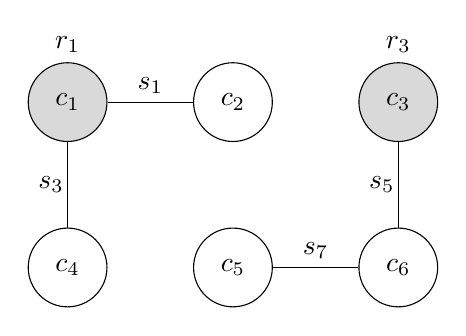
\begin{tikzpicture}[x=1.5cm,y=1.5cm,scale=0.7]

 % 設定
 \tikzset{root/.style={circle,draw=black,fill=gray!30,minimum size=1cm}}
 \tikzset{node/.style={circle,draw=black,minimum size=1cm}}
 
 % 補助線
 % \draw [help lines,blue,step=2cm] (-3,0) grid (3,-3);

 % 時間 %
 % \node[rectangle,draw=black] at (-3,1) {$t=0$};

 % root %
 \node[root] at (-2,0) (1){$c_1$};
 \node[above=0.5cm] at (1) {$r_1$};
 \node[root] at (2,0) (3){$c_3$};
 \node[above=0.5cm] at (3) {$r_3$};

 % node %
 \node[node] at (0,0) (2){$c_2$};
 \node[node] at (-2,-2) (4){$c_4$};
 \node[node] at (0,-2) (5){$c_5$};
 \node[node] at (2,-2) (6){$c_6$};

 % 繋がっていない辺は破線
 %\foreach \u / \v in {2/3, 2/5, 4/5}
 %\draw [dashed] (\u) -- (\v);
 % 繋がってる辺は実線
 \foreach \u / \v in {1/2, 1/4, 3/6, 5/6}
 \draw (\u) -- (\v);

 % スイッチ switch %
  \node at (-1,0.2) {$s_1$};
 % \node at (1,0.2) {$s_2$};
  \node at (-2.2,-1) {$s_3$};
 % \node at (-0.2,-1) {$s_4$};
  \node at (1.8,-1) {$s_5$};
 % \node at (-1,-1.8) {$s_6$};
  \node at (1,-1.8) {$s_7$};
 %

\end{tikzpicture}

%%%%%%%%%%%%%%%%%%%%%%%%%%%%%%%%%%%%%%%%%%%%%%%%%%%%%%%%%%
%%% Local Variables:
%%% mode: japanese-latex
%%% TeX-master: paper.tex
%%% End:
}
   & \onslide<2> \lw{$\Rightarrow$} & 
	\onslide<2> \scalebox{0.8}{%%%%%%%%%%%%%%%%%%%%%%%%%%%%%%%%%%%%%%%%%%%%%%%%%%
% 実行例(t=1) (第6章で使う)
%%%%%%%%%%%%%%%%%%%%%%%%%%%%%%%%%%%%%%%%%%%%%%%%%%

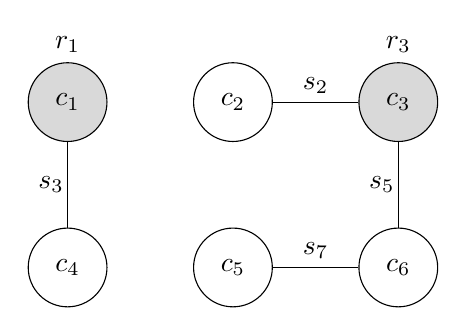
\begin{tikzpicture}[x=1.5cm,y=1.5cm,scale=0.7]

 % 設定
 \tikzset{root/.style={circle,draw=black,fill=gray!30,minimum size=1cm}}
 \tikzset{node/.style={circle,draw=black,minimum size=1cm}}
 
 % 補助線
 % \draw [help lines,blue,step=2cm] (-3,0) grid (3,-3);

 % 時間 %
 % \node[rectangle,draw=black] at (-3,1) {$t=1$};

 % root %
 \node[root] at (-2,0) (1){$c_1$};
 \node[above=0.5cm] at (1) {$r_1$};
 \node[root] at (2,0) (3){$c_3$};
 \node[above=0.5cm] at (3) {$r_3$};

 % node %
 \node[node] at (0,0) (2){$c_2$};
 \node[node] at (-2,-2) (4){$c_4$};
 \node[node] at (0,-2) (5){$c_5$};
 \node[node] at (2,-2) (6){$c_6$};

 % 繋がっていない辺は破線
 %\foreach \u / \v in {2/3, 2/5, 4/5}
 %\draw [dashed] (\u) -- (\v);
 % 繋がってる辺は実線
 \foreach \u / \v in {2/3, 1/4, 3/6, 5/6}
 \draw (\u) -- (\v);

 % スイッチ switch %
 % \node at (-1,0.2) {$s_1$};
 %
 \node at (1,0.2) {$s_2$};
 \node at (-2.2,-1) {$s_3$};
 % \node at (-0.2,-1) {$s_4$};
 \node at (1.8,-1) {$s_5$};
 % \node at (-1,-1.8) {$s_6$};
 \node at (1,-1.8) {$s_7$};
 %

\end{tikzpicture}

%%%%%%%%%%%%%%%%%%%%%%%%%%%%%%%%%%%%%%%%%%%%%%%%%%%%%%%%%%
%%% Local Variables:
%%% mode: japanese-latex
%%% TeX-master: paper.tex
%%% End:
}\\
   & & \onslide<2> \lower1ex\hbox{$\Downarrow$} \\
   & & \\
   \onslide<1-> \scalebox{0.8}{%%%%%%%%%%%%%%%%%%%%%%%%%%%%%%%%%%%%%%%%%%%%%%%%%%
% 実行例(t=3) (第6章で使う)
%%%%%%%%%%%%%%%%%%%%%%%%%%%%%%%%%%%%%%%%%%%%%%%%%%
\begin{tikzpicture}[scale=0.6]

 % 設定
 \tikzset{node/.style={circle,draw=black,fill=white}}

 \definecolor{edge1}{RGB}{191,0,0}
 \definecolor{node1}{RGB}{249,200,200}
 \definecolor{edge3}{RGB}{38,38,134}
 \definecolor{node3}{RGB}{200,200,249}

 % 補助線
 % \draw [help lines,blue] (0,0) grid (20,6);

 % node %
 \node[circle, ultra thick, draw=edge1, fill=node1](out1){1};
 \node[node, fill=node3, right=of out1] (out2){2};
 \node[circle, ultra thick, draw=edge3,fill=node3, right=of out2](out3){3};
 \node[node, fill=node3, below=of out1] (out4){4};
 \node[node, fill=node3, below=of out2] (out5){5};
 \node[node, fill=node3, below=of out3] (out6){6};

 \foreach \u / \v in {}
 \draw [very thick, edge1] (\u) -- (\v);

 \foreach \u / \v in {out2/out3,out2/out5,out4/out5,out5/out6}
 \draw [very thick, edge3](\u) -- (\v);
\end{tikzpicture}

%%%%%%%%%%%%%%%%%%%%%%%%%%%%%%%%%%%%%%%%%%%%%%%%%%%%%%%%%%
%%% Local Variables:
%%% mode: japanese-latex
%%% TeX-master: paper.tex
%%% End:
}
   & \onslide<2> \lw{$\Leftarrow$} &
   \onslide<2> \scalebox{0.8}{%%%%%%%%%%%%%%%%%%%%%%%%%%%%%%%%%%%%%%%%%%%%%%%%%%
% 実行例(t=2) (第6章で使う)
%%%%%%%%%%%%%%%%%%%%%%%%%%%%%%%%%%%%%%%%%%%%%%%%%%

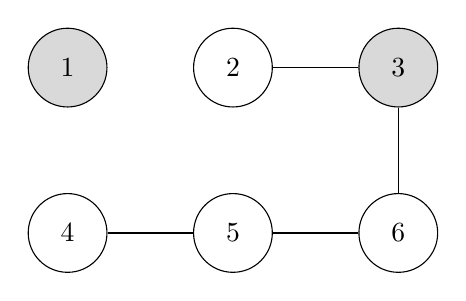
\begin{tikzpicture}[x=1.5cm,y=1.5cm,scale=0.7]

 % 設定
 \tikzset{root/.style={circle,draw=black,fill=gray!30,minimum size=1cm}}
 \tikzset{node/.style={circle,draw=black,minimum size=1cm}}
 
 % 補助線
 % \draw [help lines,blue,step=2cm] (-3,0) grid (3,-3);

 % 時間 %
 % \node[rectangle,draw=black] at (-3,1) {$t=2$};

 % root %
 \node[root] at (-2,0) (1){$1$};
% \node[above=0.5cm] at (1) {$r_1$};
 \node[root] at (2,0) (3){$3$};
 %\node[above=0.5cm] at (3) {$r_3$};

 % node %
 \node[node] at (0,0) (2){$2$};
 \node[node] at (-2,-2) (4){$4$};
 \node[node] at (0,-2) (5){$5$};
 \node[node] at (2,-2) (6){$6$};

 % 繋がっていない辺は破線
 %\foreach \u / \v in {2/3, 2/5, 4/5}
 %\draw [dashed] (\u) -- (\v);
 % 繋がってる辺は実線
 \foreach \u / \v in {2/3, 4/5, 3/6, 5/6}
 \draw (\u) -- (\v);

 % スイッチ switch %
 % \node at (-1,0.2) {$s_1$};
 % \node at (1,0.2) {$s_2$};
 % \node at (-2.2,-1) {$s_3$};
 % \node at (-0.2,-1) {$s_4$};
 % \node at (1.8,-1) {$s_5$};
 % \node at (-1,-1.8) {$s_6$};
 % \node at (1,-1.8) {$s_7$};
 %

\end{tikzpicture}

%%%%%%%%%%%%%%%%%%%%%%%%%%%%%%%%%%%%%%%%%%%%%%%%%%%%%%%%%%
%%% Local Variables:
%%% mode: japanese-latex
%%% TeX-master: paper.tex
%%% End:
}\\
   \onslide<1->$t= \only<1>{\ ?} \only<2>{\structure{\bf 3}} $ (ゴール状態) 
   & & \onslide<2> $t=2$
  \end{tabular}
 \end{figure}
\end{exampleblock}
\end{frame}

\backupend

%%% Local Variables:
%%% mode: japanese-latex
%%% TeX-master: "slide.tex"
%%% End:
